\chapter{Clustering}

Nous avons expérimentés plusieurs méthodes de clustering pour extraire des points d’intérêts à partir des données
des quelques 80 000 photos que nous possédons.

Nous présentons dans cette partie les méthodes que nous avons utilisées, leur pertinence dans le cadre de ce projet, et
autres avantages et/ou inconvénients.

Nous avons principalement fais un clustering basé sur la latitude/longitude. Nous montrons néanmoins (dans la partie \textit{K-Means}) qu'un clustering sur d'autres critères, par exemple le mois de prise de la photo, ne donne pas de résultats satisfaisant.

\section{Validation des méthodes de clustering}
    Avant de voir ces méthodes de clustering, une question se pose~: comment valider la qualité de ces clusters.

    La notion de ``point d’intérêt'' est dure à quantifier. En effet, comment savoir si un point d’intérêt n'est pas si
    intéressant que ça au final ? Comment savoir qu'un point d’intérêt en cache en réalité plusieurs ?

    Si ces points là sont durs à quantifier, on peut néanmoins prendre en compte ces facteurs~:

    \begin{enumerate}
        \item \textbf{Le nombre de clusters} Même si Lyon n'est peut-être pas aussi vivante que New York ou Milan, si
        une méthode nous donne 5 points d’intérêts sur tout le Grand Lyon, c'est qu'elle n'est pas pertinente.
        \item \textbf{La taille des clusters} Si un cluster couvre la moitié de la ville, c'est généralement que l'algorithme
        a du mal à séparer des points d’intérêt proches.
        \item \textbf{La densité des clusters} Globalement, la densité doit être bien distribuée. Les clusters
        doivent aussi être relativement denses.
    \end{enumerate}

    L'évaluation de ces critères est facilitée par les outils mis à disposition par Knime et pandas, mais souvent l'observation
    manuelle reste nécessaire pour paramétrer certaines méthodes afin qu'elles donnent un bon résultat.


\section{Clustering hiérarchique}
    Cette méthode, bien qu'utile quand on ne connaît pas le nombre de clusters
    attendu (comme c'est le cas dans ce projet), ne passe pas à l'échelle~:
    son exécution sur la totalité du jeu de donnée provoque un dépassement de mémoire.

    Nous avons malgré tout réalisé un échantillonnage aléatoire (de 1,000 lignes)
    de notre jeu de données sur lequel on a effectué un \textit{clustering hiérarchique}
    afin d'avoir une idée sur le nombre de clusters qui pouvaient être extraits.

    \begin{figure}[H]
        \centering
        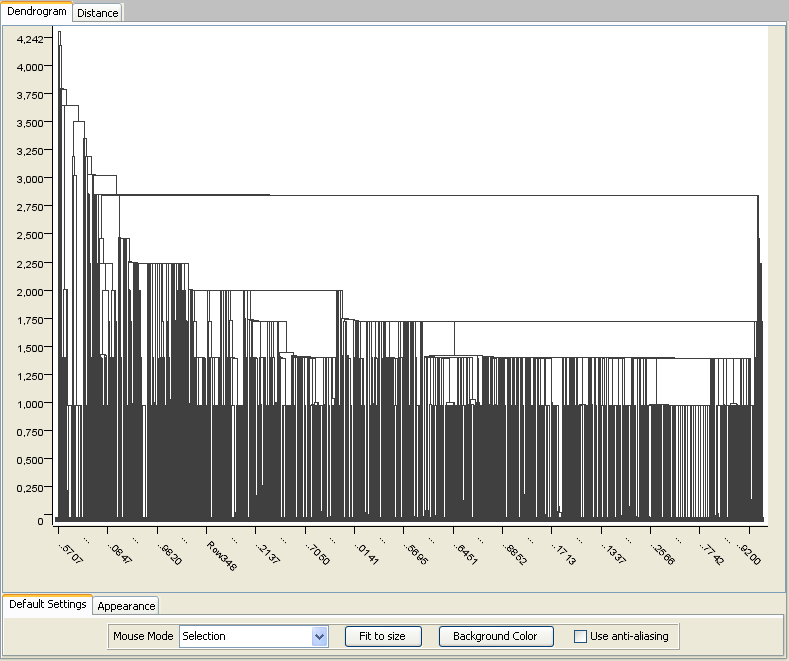
\includegraphics[scale=0.3]{../screenshots/hierarchical_clustering_1000_samples.png}
        \caption{Résultat du clustering hiérarchique sur 1000 échantillons}
        \label{diagram:hierarchical_clustering_1000_samples}
    \end{figure}

    Mais même sur un jeu de données aussi restreint (par rapport aux données
    originales), le résultat était difficilement exploitable (car très dense),
    et le fait que les données exploitées représentaient moins de $5\%$ des
    données originales faisait que ce clustering était fort instable (structure
    variant sur des samplings différents).

\section{K-Means}
    Bien que plus rapide à l’exécution que le clustering hiérarchique (et moins demandant en ressources mémoire),
    le clustering \textit{K-Means} n'est pas des plus adaptés pour ce projet~: il demande de connaître le nombre de clusters et
    donne des clusters parfois répartis sur de grandes zones et moins denses que ce que donnent d'autres méthodes (notamment Mean Shift). La densité des clusters est aussi très disparate~: on peut se retrouver avec un cluster contenant 70\% des photos.

    \begin{figure}[H]
        \centering
        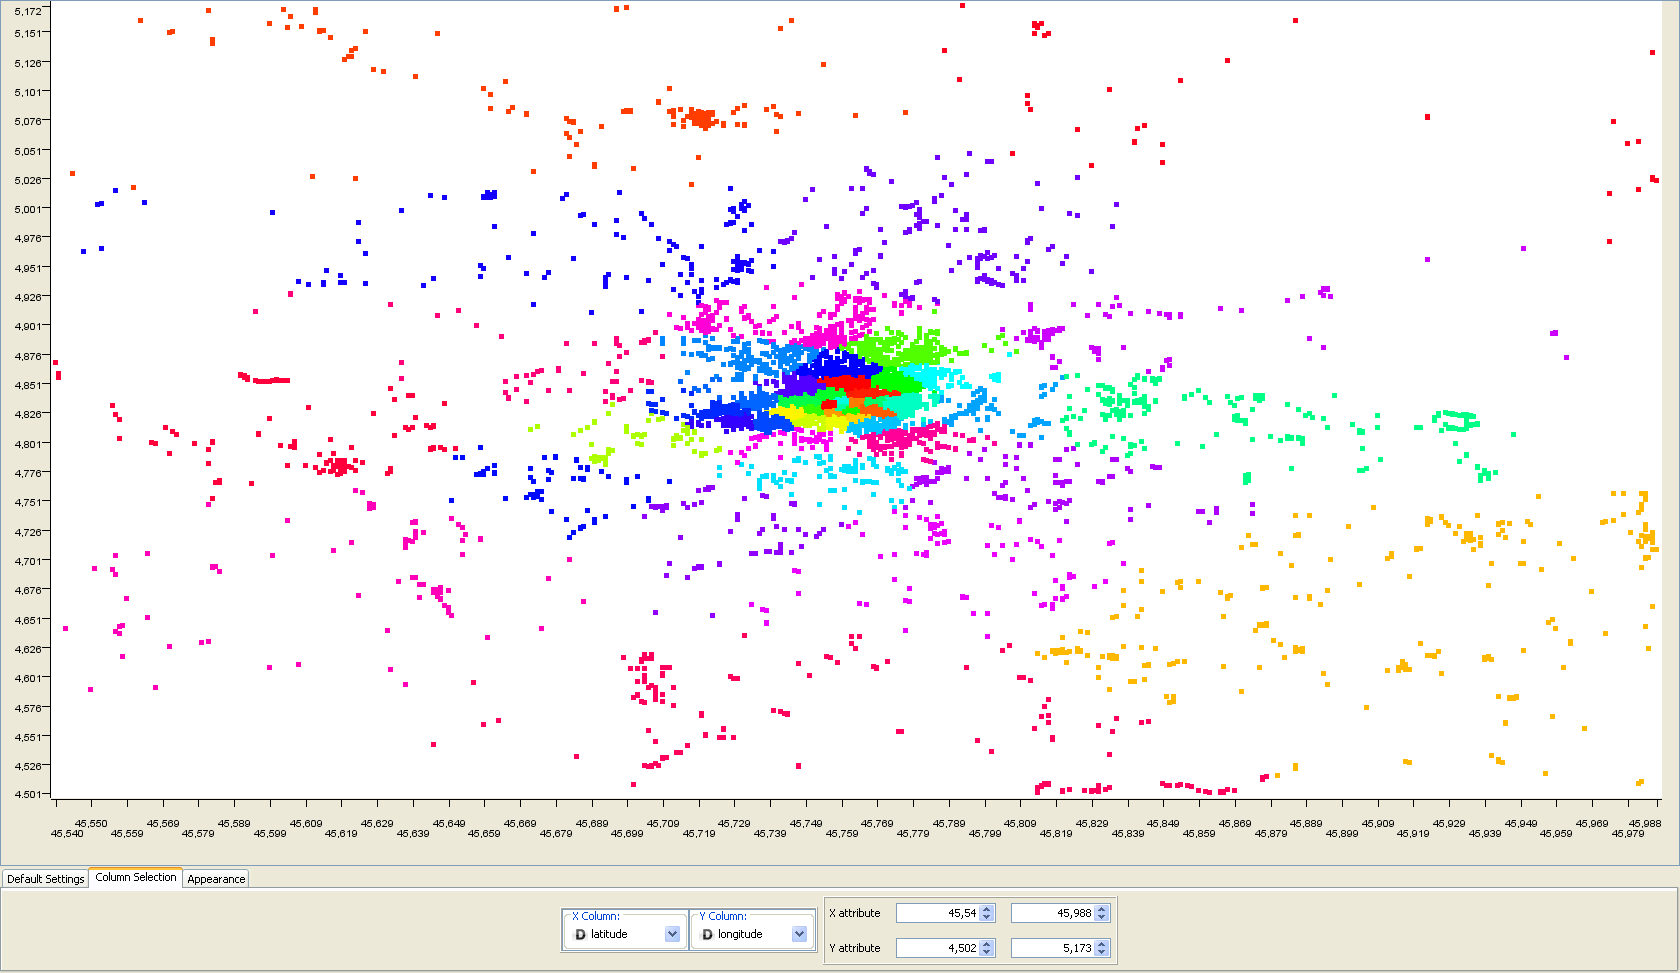
\includegraphics[scale=0.25]{../screenshots/kmeans_geographic.png}
        \caption{Résultat du clustering \textit{K-Means}}
        \label{diagram:kmeans_geographic}
    \end{figure}

    Nous avons aussi essayé de réaliser des clusters en nous basant sur le mois de prise des photos, afin de montrer certaines tendances (quartier plus fréquentés pendant l'été, par exemple) mais les résultats étaient peu satisfaisants (pas de correlation particulière entre le mois de prise de la photo et sa position).

    \begin{figure}[H]
        \centering
        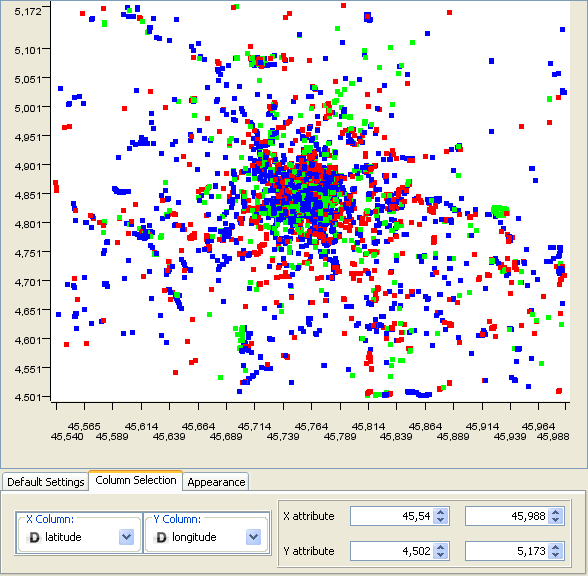
\includegraphics[scale=0.28]{../screenshots/kmeans_month.png}
        \caption{Résultat du clustering \textit{K-Means} basé sur la date de prise des photos}
        \label{diagram:kmeans_month}
    \end{figure}


\section{DBScan}
    DBScan cumule les tares de \textit{K-Means} et du clustering hiérarchique : très lent à s’exécuter (avec dépassement mémoire
    si on utilise la totalité du jeu de données) et donnant des clusters très dispersés et même moins denses que ceux de \textit{K-Means}.


    \begin{figure}[H]
        \centering
        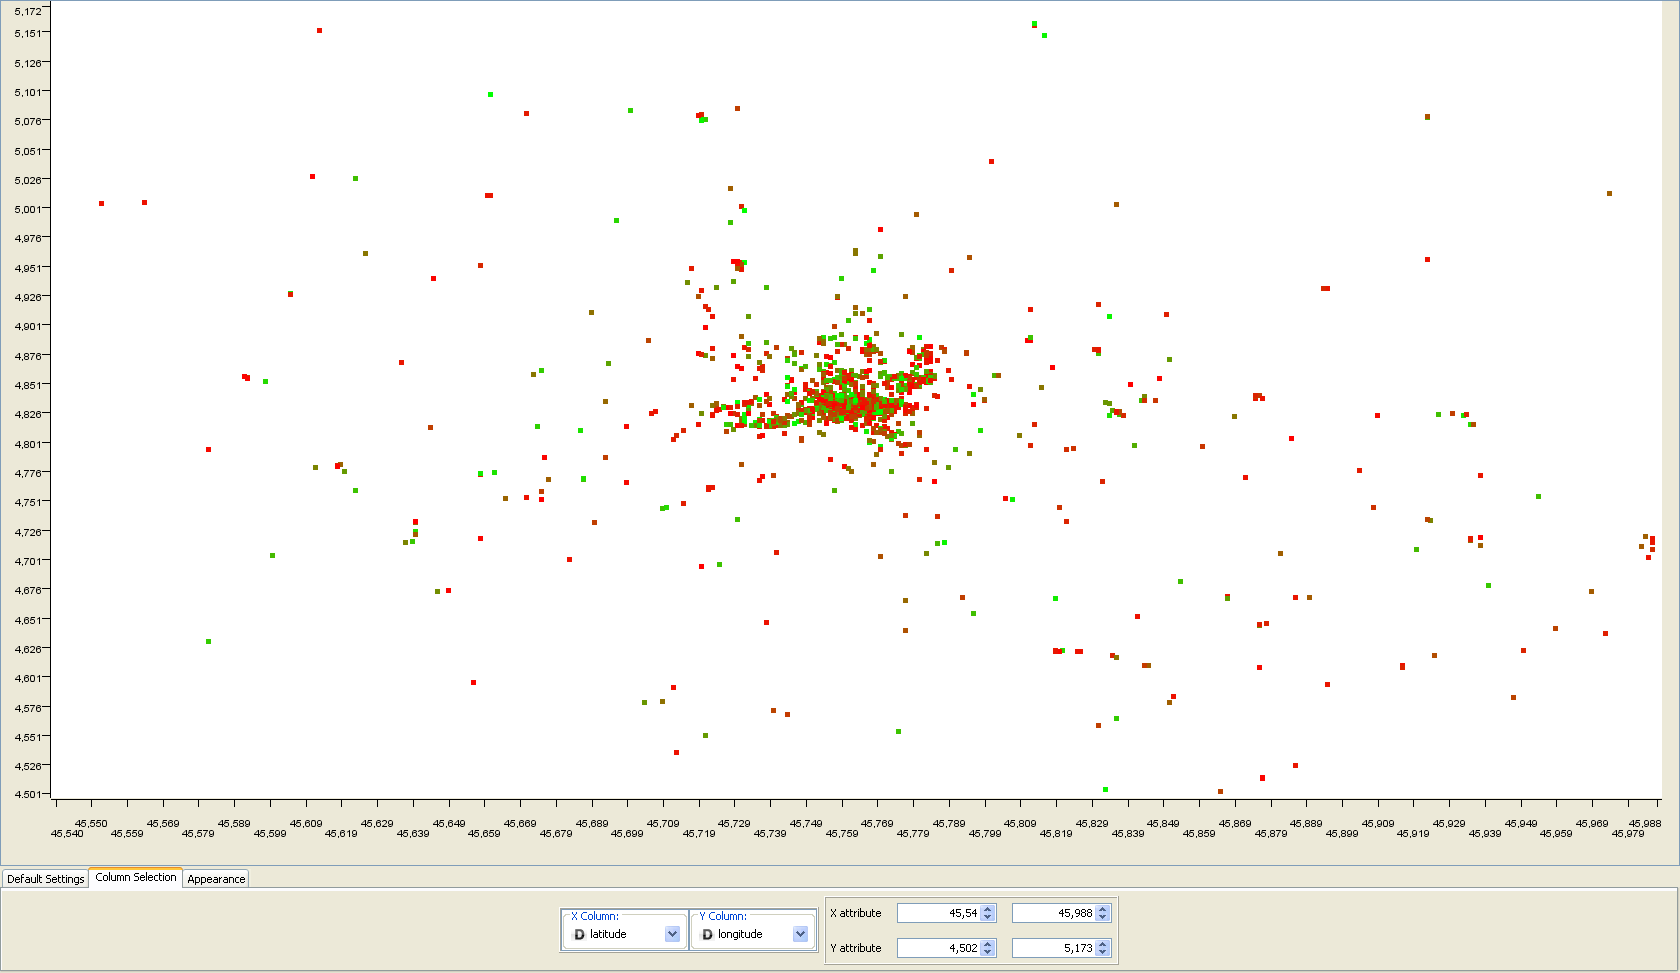
\includegraphics[scale=0.3]{../screenshots/dbscan_geographic.png}
        \caption{Résultat du clustering avec DBScan}
        \label{diagram:dbscan_geographic}
    \end{figure}


\section{Mean Shift}
    L'algorithme \textit{Mean Shift} est celui qui nous a donné les meilleurs résultats : Un grand nombre (autour de 360) clusters denses,
    à la taille réduite et ayant une densité relativement homogène (pas de grand point d’intérêt à 30 000 photos et d'autres à 2 photos
    comme c'était le cas pour \textit{K-Means}).

    \begin{figure}[H]
        \centering
        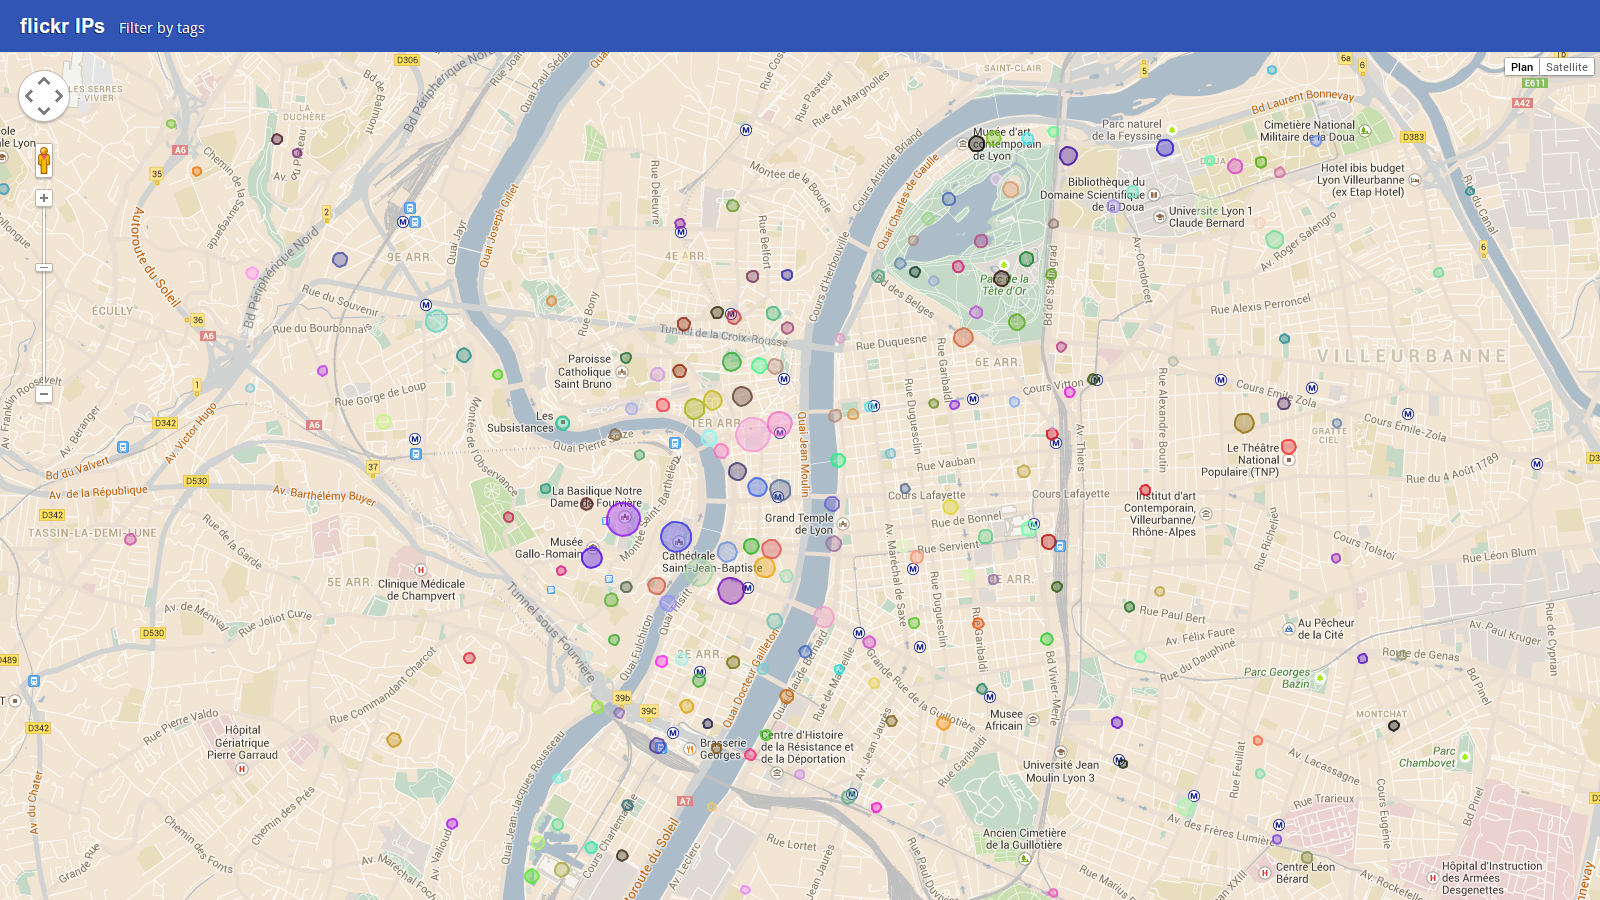
\includegraphics[scale=0.3]{../screenshots/ui-global.png}
        \caption{Résultat du clustering avec MeanShift, vu depuis l'application web}
        \label{diagram:ui-global-clustering}
    \end{figure}
